Chương này trình bày những kiến thức cơ sở để triển khai luận văn này, gồm:
\begin{itemize}
\item Kiểm thử phần mềm,
\item Sinh ngẫu nhiên dữ liệu thử,
\item Kỹ thuật Dynamic Symbolic Execution.
\end{itemize}

\section{Kiểm thử phần mềm}

\cite{myers2011art,whittaker2000software,ammann2016introduction}

\subsection{Giới thiệu}
Trong nền kinh tế hiện nay, ngành công nghiệp phần mềm giữ vai trò hết sức quan trọng. Với một số nước có nền công nghệ thông tin phát triển thì ngành công nghiệp phần mềm có khả năng chi phối cả nền kinh tế. Tuy nhiên để đảm bảo chất lượng cho các phần mềm là một thách thức không nhỏ trong ngành công nghiệp phần mềm. Việc phát hiện và khắc phục các lỗi cho các phần mềm là một công việc đòi hỏi nhiều nỗ lực và chi phí trong phát triển phần mềm. Với những lĩnh vực ứng dụng ngày càng mở rộng của phần mềm hiện nay thì  một sản phẩm phần mềm có thể được nhiều người sử dụng biết đến, nó mang lại hiệu quả tích cực trong công việc của người sử dụng. Tuy nhiên, một phần mềm lỗi sẽ ảnh hưởng đến người sử dụng, gây thiệt hại về kinh tế cũng như ảnh hưởng đến tiến độ công việc của người sử dụng. Phần mềm phải luôn đảm bảo được sự ổn định, không phát sinh lỗi, tránh gây ảnh hưởng tới người sử dụng.

Việc kiểm thử phần mềm chính là một quá trình hoặc một loạt các quy trình được thiết kế, để đảm bảo mã máy tính chỉ làm những gì nó được thiết kế và nó không làm bất cứ điều gì ngoài ý muốn \cite{myers2011art}. Phần mềm phải được dự đoán, nhất quán và không gây bất ngờ cho người dùng. Đây là một bước quan trọng trong quá trình phát triển một phần mềm, giúp cho người phát triển phần mềm và người sử dụng thấy được hệ thống đã đáp ứng yêu cầu đặt ra.

\subsection{Các phương pháp kiểm thử}
\textbf{\textit{Kiểm thử tĩnh (Static testing)}}: Là phương pháp kiểm thử phần mềm bằng cách duyệt lại các yêu cầu và các đặc tả bằng tay, thông qua việc sử dụng giấy, bút để kiểm tra tính logic từng chi tiết mà không cần chạy chương trình. Kiểu kiểm thử này thường được sử dụng bởi chuyên viên thiết kế, người viết mã lệnh chương trình. Kiểm thử tĩnh cũng có thể được tự động hóa bằng cách thực hiện kiểm tra toàn bộ hệ thống thông qua một trình thông dịch hoặc trình biên dịch, xác nhận tính hợp lệ về cú pháp của chương trình.
		
\textbf{\textit{Kiểm thử động (Dynamic testing)}}: Là phương pháp kiểm thử thông qua việc chạy chương trình để điều tra trạng thái tác động của chương trình, dựa trên các ca kiểm thử xác định các đối tượng kiểm thử của chương trình. Đồng thời kiểm thử động sẽ tiến hành kiểm tra cách thức hoạt động của mã lệnh, tức là kiểm tra phản ứng từ hệ thống với các biến luôn thay đổi theo thời gian. Trong kiểm thử động, phần mềm phải được biên dịch và chạy, và bao gồm việc nhập các giá trị đầu vào và kiểm tra giá trị đầu ra có như mong muốn hay không.	
	
\subsection{Các chiến lược kiểm thử}

Trong chiến lược kiểm thử, đề tài quan tâm đến hai chiến lược kiểm thử đó là kiểm thử hộp đen, kiểm thử hộp trắng.
	
\textbf{\textit{Kiểm thử hộp đen – Black box}}. Đây là một trong những cách kiểm thử quan trọng, cách thức hoạt động chủ yếu dựa vào hướng dữ liệu inputs/ouputs của chương trình, xem chương trình như là một “hộp đen” và hoàn toàn không quan tâm về cách xử lý, cũng như cấu trúc bên trong của chương trình. Kiểm thử hộp đen tập trung vào tìm các trường hợp mà chương trình không thực hiện theo các đặc tả kỹ thuật. Kiểm thử viên hộp đen sẽ cố gắng tìm ra những lỗi mà những lập trình viên không tìm ra. Nhưng phương pháp kiểm thử này cũng có mặt hạn chế của nó, kiểm thử viên không biết các phần mềm được kiểm tra thực sự được xây dựng như thế nào, cố gắng viết rất nhiều ca kiểm thử để kiểm tra một thứ gì đó mà đáng lẽ chỉ cần kiểm tra bằng một ca kiểm thử duy nhất, hoặc một số phần của chương trình có thể bị bỏ qua không được kiểm tra.
		
Do vậy, kiểm thử hộp đen có ưu điểm là đánh giá khách quan, mặt khác nó lại có nhược điểm là thăm dò mù. Trong phần nghiên cứu của đề tài, kiểm thử hộp đen cũng được sử dụng như một phương pháp đo độ tương tự hành vi của các chương trình.
		
\textbf{\textit{Kiểm thử hộp trắng – White box}}. Đây là một chiến lược kiểm thử khác, trái ngược hoàn toàn với kiểm thử hộp đen, kiểm thử hộp trắng hay còn gọi là kiểm thử hướng logic của phần mềm. Cách kiểm thử này cho phép tạo ra dữ liệu thử nghiệm từ việc kiểm tra, khảo sát cấu trúc bên trong và kiểm thử tính logic của chương trình. Dữ liệu thử nghiệm có độ phủ lớn, đảm bảo được tất cả các đường dẫn, hoặc các nhánh của chương trình được thực hiện ít nhất một lần, khắc phục được những nhược điểm thăm dò mù trong cách kiểm thử hộp đen.
		
Phương pháp kiểm thử hộp trắng cũng có thể được sử dụng để đánh giá một bộ kiểm thử được tạo với các phương pháp kiểm thử hộp đen. Trong các phép đo độ tương tự của đề tài, phương pháp kiểm thử hộp trắng là một phương pháp quan trọng, được áp dụng để đo hành vi của các chương trình.
	
\subsection{Các cấp độ kiểm thử trong kiểm thử phần mềm}
Kiểm thử phần mềm gồm có các cấp độ: 
\begin{itemize}
	\item Kiểm thử đơn vị
	\item Kiểm thử tích hợp
	\item Kiểm thử hệ thống
	\item Kiểm thử chấp nhận sản phẩm
\end{itemize}
	
\begin{center}
	\begin{figure}[htp]
		\begin{center}
			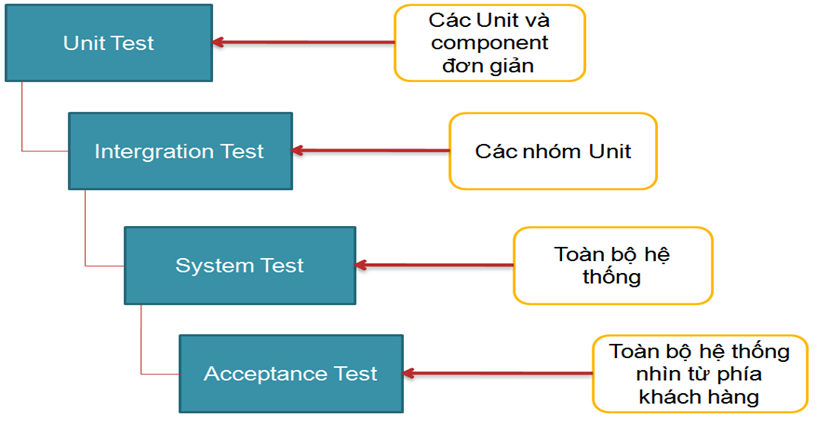
\includegraphics[scale=.3]{giai-doan-kiem-thu-1.png}
		\end{center}
		\caption{Sơ đồ các cấp độ kiểm thử}
		\label{refhinh1}
	\end{figure}
\end{center}
	
\subsection{Đảm bảo chất lượng phần mềm}
\textbf{Định nghĩa theo Daniel Galin \cite{galin2004software}:} Đảm bảo chất lượng phần mềm là một tập hợp các hành động được lên kế hoạch một cách hệ thống để cung cấp đầy đủ niềm tin rằng quá trình phát triển phần mềm phù hợp để thành lập các yêu cầu chức năng kỹ thuật cũng như các yêu cầu quản lý theo lịch trình và hoạt động trong giới hạn.


\section{Sinh ngẫu nhiên dữ liệu thử}
%Phần này trình bày cơ bản về sinh dữ liệu thử ngẫu nhiên, những ưu và nhược điểm cùng những cải tiến để nâng cao hiệu quả.
Sinh ngẫu nhiên dữ liệu thử là một kỹ thuật kiểm thử phần mềm Black-Box kỹ thuật này tạo ra ngẫu nhiên các giá trị đầu vào và thực thi từng giá trị đầu vào này trên chương trình được kiểm thử. Kết quả của đầu ra được so sánh với các thông số kỹ thuật của phần mềm, để xác định đầu ra thử nghiệm thành công hoặc không thành công \cite{myers2011art}.  

Kỹ thuật này không quan tâm đến hành vi và cấu trúc bên trong của chương trình, chỉ tập trung tìm kiếm những trường hợp chương trình không hoạt động theo đặc tả kỹ thuật của chương trình. Trong phương pháp này, dữ liệu thử nghiệm được tạo ngẫu nhiên từ các đặc tả kỹ thuật của phần mềm (tức là không liên quan tới hành vi và cấu trúc của chương trình).

\subsection*{Ví dụ:}
\lstinputlisting[caption = {Hàm sinh ngẫu nhiên dữ liệu thử}]{RandomTesting.cs}
Đây là một hàm sinh ngẫu nhiên dữ liệu thử, chúng ta thấy hàm \textbf{testAbs} chỉ thực hiện việc tạo giá trị đầu vào ngẫu nhiên \textbf{int x} theo đặc tả tham số đầu vào của chương trình \textbf{myAbs}, và kiểm tra kết quả đầu ra của chương trình \textbf{assert(result >= 0)}, không quan tâm hành vi và cấu trúc bên trong của hàm \textbf{myAbs}.

\subsection*{Ưu điểm và hạn chế}

\textit{* Ưu điểm:}
\begin{itemize}
	\item Đơn giản, dễ dàng sinh các đầu vào ngẫu nhiên
	\item Không tốn nhiều tài nguyên bộ nhớ lúc thực thi
\end{itemize}

\textit{* Hạn chế:}
\begin{itemize}
	\item Một nhánh hành vi của chương trình được kiểm thử nhiều lần với nhiều đầu vào khác nhau
	\item Có thể một số nhánh hành vi của chương trình bị bỏ qua
	\item Khó xác định khi nào việc kiểm thử nên dừng lại
	\item Không biết dữ liệu thử có duyệt được tất cả các nhánh trong chương trình hay không
\end{itemize}

\subsection*{Hướng khác phục}
Để xác định khi nào việc kiểm thử dừng lại, hệ thống kiểm thử ngẫu nhiên có thể kết hợp với các kỹ thuật Adequacy Criterion \cite{zhu1997software}. Kỹ thuật Adequacy Criterion là một kỹ thuật yêu cầu duyệt tất cả các nhánh của chương trình, bằng việc kết hợp này cho phép việc kiểm thử chỉ dừng lại khi tất cả các câu lệnh của chương trình được thực thi ít nhất một lần.

Một kỹ thuật khác giúp khắc phục được hạn chế của kiểm thử ngẫu nhiên đó là kỹ thuật thực thi tượng trưng \cite{king1976symbolic}. Thực thi tượng trưng là một kỹ thuật xây dựng các ràng buộc dựa vào các điều kiện tại các nút nhánh của chương trình, giải quyết các ràng buộc đó để sinh ra các giá trị  đầu của chương trình. Thực thi các giá trị đầu vào này, chúng ta có thể duyệt được tất cả các nhánh của chương trình. 


\section{Kỹ thuật Dynamic symbolic execution}
% What? 
% why?
% how?
% who?

Dynamic symbolic execution (DSE) là một kỹ thuật duyệt tự động tất cả các đường đi có thể của chương trình bằng cách chạy chương trình với nhiều giá trị đầu vào khác nhau để tăng độ phủ của dữ liệu thử \cite{xie2009fitness}.

Dựa trên các tham số đầu vào của chương trình, DSE sẽ tạo ra các giá trị đầu vào cụ thể và thực thi chương trình với các giá trị cụ thể này. Trong quá trình thực thi, DSE sẽ ghi nhận lại ràng buộc tại các nút, phủ định lại các ràng buộc này và sinh các giá trị đầu vào thỏa điều kiện ràng buộc tại các nút rẽ nhánh này. Với một giá trị đầu vào cụ thể, DSE sẽ thực thi chương trình và duyệt được một đường đi cụ thể, quá trình thực thi này sẽ lặp lại cho đến khi duyệt hết tất cả các đường đi của chương trình.

\subsection*{Thuật toán}
\begin{center}
	\begin{figure}[htp]
		\begin{center}
			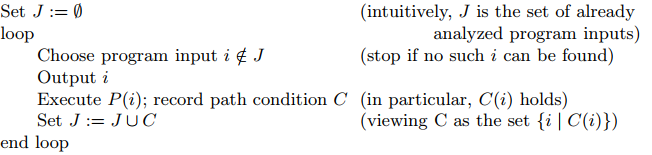
\includegraphics[scale=.7]{thuat_toan_DSE.png}
		\end{center}
		\caption{Thuật toán kỹ thuật DSE}
		\label{refhinh1}
	\end{figure}
\end{center}


\subsection*{Ví dụ:}

\lstinputlisting[caption = {Minh họa kỹ thuật DSE}]{DSE.cs}
	
Trong ví dụ trên, chúng ta xem xét hàm \textbf{test\_me} với hai tham số đầu vào là \textbf{int x} và \textbf{int y}, và hàm này không có giá trị trả về. Cách thức làm việc của DSE trên hàm \textbf{test\_me} như sau: 

Đầu tiên, DSE tạo hai giá trị đầu vào ngẫu nhiên \textbf{x} và \textbf{y}, giả sử \textbf{x = 22} và \textbf{y = 7}. Ngoài ra, DSE sẽ theo dõi trạng thái các giá trị đầu vào của chương trình: \textbf{x} bằng một tham số \textbf{x\_0} và \textbf{y} bằng một tham số \textbf{y\_0}.

Ở dòng đầu tiên, số nguyên \textbf{z} được gán bằng hàm \textbf{foo(y)}. Điều này có nghĩa là \textbf{z} bây giờ bằng 14, và ở trạng thái tượng trưng, biến \textbf{z} có giá trị \textbf{2*y\_0}. 

Tại điểm nhánh \textbf{“z == x”}, DSE nhận biết giá trị của \textbf{x} không bằng giá trị của \textbf{z}. Về mặt biểu tượng, DSE lưu trữ ràng buộc này là \textbf{(z != x)}, và điều kiện đường dẫn sẽ là: \textbf{2*y\_0 != x\_0}. DSE sau đó đi theo nhánh “\textbf{false}” dẫn đến kết thúc chương trình.

Sau khi kết thúc chương trình, DSE sẽ quay trở lại điểm nhánh gần nhất và cố gắng chọn nhánh "true". Với mục đích này, nó phủ định ràng buộc được thêm gần nhất trong điều kiện đường dẫn \textbf{2*y\_0 != x\_0} thành \textbf{2*y\_0 == x\_0}. Để thỏa mãn ràng buộc \textbf{2*y\_0 != x\_0}, hai số nguyên thỏa mãn ràng buộc này được trả về là \textbf{x\_0 = 2 }và\textbf{ y\_0 = 1}.


\begin{center}
	\begin{figure}[htp]
		\begin{center}
			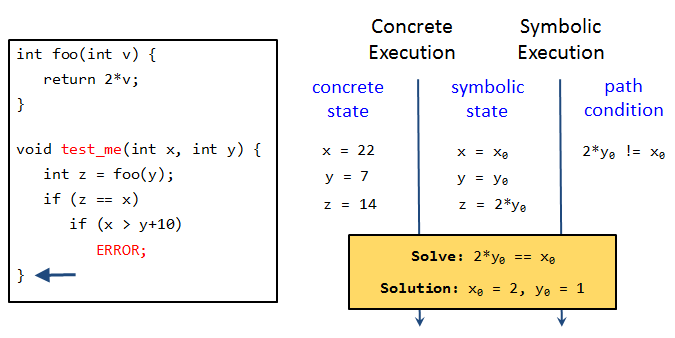
\includegraphics[scale=.4]{dse2.png}
		\end{center}
		\caption{Các giá trị DSE sinh ra sau khi thực thi chương trình lần 1}
		\label{refhinh1}
	\end{figure}
\end{center}

Sau đó, DSE khởi động lại hàm \textbf{test\_me}, lần này nó gọi các giá trị đầu vào cụ thể được tạo ra bởi quá trình giải quyết ràng buộc: \textbf{x = 2} và \textbf{y = 1}. DSE tiếp tục theo dõi trạng thái các biến với \textbf{x = x\_0} và \textbf{y = y\_0}.

Sau khi thực hiện dòng đầu tiên, \textbf{z} có giá trị cụ thể 2 và giá trị biểu tượng 2*y\_0\textbf{}.

Ở dòng kế tiếp, chúng ta kiểm tra tình trạng nhánh \textbf{z == x}. Trong trường hợp này, điều kiện là đúng, vì vậy điều kiện đường dẫn của chúng ta trở thành \textbf{2*y\_0 == x\_0}. Sau đó \textbf{DSE} kiểm tra dòng tiếp theo của nhánh \textbf{"true"}.

Tại điểm nhánh tiếp theo, \textbf{x} có giá trị cụ thể là 2 và \textbf{y + 10} có giá trị cụ thể là 11, vì vậy \textbf{DSE} lấy nhánh \textbf{"false"}, kết thúc chương trình. Thêm ràng buộc tượng trưng \textbf{x\_0 <= y\_0 + 10} vào điều kiện đường dẫn, là sự phủ định của điều kiện nhánh mà \textbf{DSE} phát hiện là \textbf{fasle}.

Vì DSE đã đến cuối chương trình, nó phủ nhận ràng buộc được thêm gần nhất trong điều kiện đường dẫn để có được \textbf{x\_0> y\_0 + 10}, và sau đó nó vượt qua các ràng buộc \textbf{2*y\_0 == x AND x\_0> y\_0 + 10}. Để thỏa những ràng buộc này, \textbf{DSE} trả về \textbf{x\_0 = 30} và \textbf{y\_0 = 15}.

\begin{center}
	\begin{figure}[htp]
		\begin{center}
			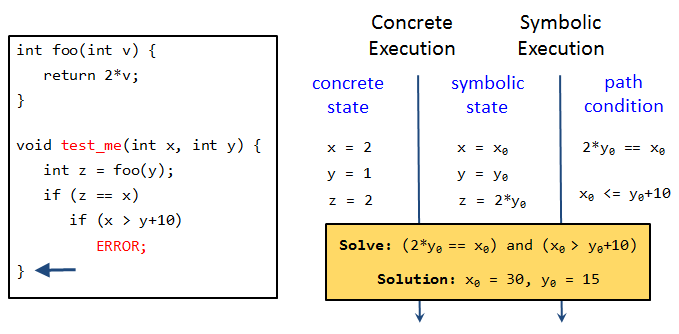
\includegraphics[scale=.4]{dse3.png}
		\end{center}
		\caption{Các giá trị DSE sinh ra sau khi thực thi chương trình lần 2}
		\label{refhinh1}
	\end{figure}
\end{center}

Bây giờ, DSE chạy hàm \textbf{test\_me} một lần nữa, lần này với các đầu vào \textbf{x = 30} và \textbf{y = 15}. Trạng thái biểu tượng các biến bắt đầu \textbf{x = x\_0} và \textbf{y = y\_0}. \textbf{z} được gán giá trị cụ thể 30, trong khi giá trị ký hiệu của nó là \textbf{2*y\_0}, như trước những lần chạy trước.

Khi tới điều kiện rẻ nhánh \textbf{"z == x"}, DSE nhận thấy đây là điều kiện \textbf{true}, vì vậy DSE thêm điều kiện tượng trưng \textbf{2*y\_0 == x\_0}.

Sau đó, tại điểm nhánh tiếp theo, giá trị cụ thể của \textbf{x > y + 10}, vì vậy DSE thêm ràng buộc tượng trưng mới \textbf{x\_0 > y\_0 + 10}. Nhánh này dẫn đến \textbf{"ERROR"}, tại thời điểm đó chúng ta đã xác định được đầu vào cụ thể làm cho chương trình\textbf{"ERROR"} là: \textbf{x = 30} và \textbf{y = 15}.

\begin{center}
	\begin{figure}[htp]
		\begin{center}
			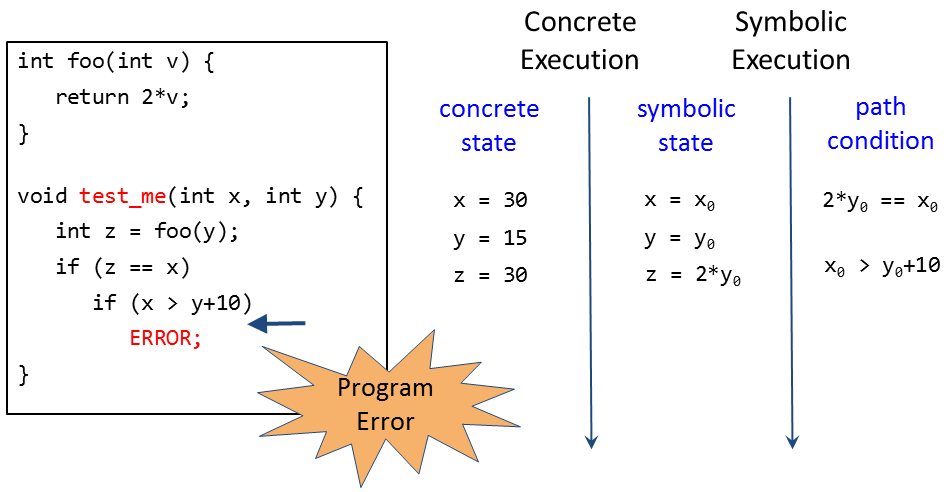
\includegraphics[scale=.4]{dse4.png}
		\end{center}
		\caption{Các giá trị DSE sinh ra sau khi thực thi chương trình lần 3}
		\label{refhinh1}
	\end{figure}
\end{center}

Kết quả, sau 3 lần chạy chương trình, DSE tạo ra được các cặp giá trị đầu vào có thể duyệt hết các nhánh của chương trình \textbf{test\_me} đó là: \textbf{[22,7], [2,1], [30,15]}
	
\subsection{Một số công cụ ứng dụng DSE}	
Hiện nay, trên thế giới có nhiều công cụ sử dụng kỹ thuật DSE để giải quyết các ràng buộc và tạo ra các giá trị đầu vào có độ phủ cao như như Pex \cite{tillmann2008pex} và SAGE \cite{godefroid2008automated}... và một công cụ có thể sử dụng được trên nhiều ngôn ngữ, nền tảng khác nhau.
		
	\begin{center}
		\begin{tabular}  {|c|c|c|} 
			\hline 
			\textbf{Tên Công cụ} & \textbf{Ngôn ngữ} & \textbf{Url} \\ 
			\hline 
			KLEE & LLVM & klee.github.io/ \\ 
			\hline 
			JPF	 & Java	& babelfish.arc.nasa.gov/trac/jpf \\
			\hline 
			jCUTE &	Java &	github.com/osl/jcute \\
			\hline 
			janala2	 & Java &	github.com/ksen007/janala2 \\
			\hline 
			JBSE	& Java	 & github.com/pietrobraione/jbse \\
			\hline 
			KeY &	Java &	www.key-project.org/ \\	
			\hline 
			Mayhem & 	Binary &	forallsecure.com/mayhem.html \\
			\hline 
			Otter &	C	& bitbucket.org/khooyp/otter/overview \\
			\hline 
			Rubyx & 	Ruby &	www.cs.umd.edu/~avik/papers/ssarorwa.pdf \\
			\hline 
			Pex	& .NET Framework	 & research.microsoft.com/en-us/projects/pex/ \\
			\hline 
			Jalangi2 &	JavaScript &	github.com/Samsung/jalangi2 \\
			\hline 
			Kite &	LLVM &	www.cs.ubc.ca/labs/isd/Projects/Kite/ \\
			\hline 
			pysymemu &	x86-64 / Native	 &github.com/feliam/pysymemu/ \\
			\hline 
			Triton	& x86 and x86-64 &	triton.quarkslab.com \\	
			\hline 
			BE-PUM &	x86	 & https://github.com/NMHai/BE-PUM	 \\	
			\hline
			
		\end{tabular} 

	\end{center}
	
\section*{Tổng kết chương}
%Tổng kết chương viết ở đây.
Chương này, trình bày khái quát và sơ lượt những kiến thức như: Kỹ thuật kiểm thử phần mềm; các kỹ thuật sinh dữ liệu thử; kỹ thuật Dynamic symbolic execution. Những kiến thức này, giúp chúng ta có cái nhìn tổng quan về cách thức kiểm thử phần mềm, giải quyết các ràng buộc trong chường trình nhằm tăng độ phủ cho các giá trị đầu vào thử nghiệm.


